% Uncomment this line for on-screen presentation
\documentclass[xcolor={dvipsnames}]{beamer}\usepackage{etoolbox}\newtoggle{printable}\togglefalse{printable}

% Uncomment this line for printable slides (disable animations and don't waste ink)
%\documentclass[handout, xcolor={dvipsnames}]{beamer}\usepackage{etoolbox}\newtoggle{printable}\toggletrue{printable}

% Adjust these for the path of the theme and its graphics, relative to this file
%\usepackage{beamerthemeFalmouthGamesAcademy}
\usepackage{../../beamerthemeFalmouthGamesAcademy}
\graphicspath{ {../../} }

% Default language for code listings
\lstset{language=C++}

\begin{document}
\title{Transition to C++ I}   
\subtitle{COMP110: Principles of Computing}

\frame{\titlepage} 

\begin{frame}
	\frametitle{Learning outcomes}
	By the end of this session you will
	\begin{itemize}
		\item Understand a thing
		\item Understand another thing
		\item Be convinced that \LaTeX\ makes better-looking slides than PowerPoint
	\end{itemize}
\end{frame}

% -------------------------------------------------------

\part{Your first C++ program}
\frame{\partpage}

\begin{frame}
	\frametitle{Project setup}
	\begin{itemize}
		\item Open \textbf{Visual Studio 2015} from the Start menu
		\item Click \textbf{New Project}
		\item Choose \textbf{Templates $\to$ Visual~C++ $\to$ Win32 $\to$ Win32~Console~Application}
		\item Choose an appropriate name and location, and click \textbf{OK}
		\item Click \textbf{Finish}
		\item When asked about source control, click \textbf{Cancel}
	\end{itemize}
\end{frame}

\begin{frame}[fragile]
	\frametitle{The code}
	\begin{itemize}
		\item Edit \texttt{$\langle$YourApplicationName$\rangle$.cpp} to match the following:
	\end{itemize}
	\begin{lstlisting}
// ConsoleApplication1.cpp : Defines the entry point for the console application.

#include "stdafx.h"
#include <iostream>

int main()
{
    std::cout << "Hello, world!" << std::endl;
    return 0;
}
	\end{lstlisting}
	\begin{itemize}
		\item Click \textbf{Debug $\to$ Start~Without~Debugging}, or press \textbf{Ctrl~+~F5}
	\end{itemize}
\end{frame}

\begin{frame}[fragile]
	\frametitle{Comments}
	\begin{lstlisting}
// ConsoleApplication1.cpp : Defines the entry point for the console application.
	\end{lstlisting}
	\begin{itemize}
		\item \lstinline{//} denotes a single-line comment
		\item Equivalent of \lstinline[language=Python]{#} in Python
		\item \textcolor{Gray}{$\hookleftarrow$} denotes a line too long to fit on the slide ---
			in your program this should be a single line
	\end{itemize}
\end{frame}

\begin{frame}[fragile]
	\frametitle{The \#include directive}
	\begin{lstlisting}
#include "stdafx.h"
#include <iostream>
	\end{lstlisting}
	\begin{itemize}
		\item \lstinline{#include} imports definitions from a \textbf{header file}
		\item Similar to \lstinline[language=Python]{import} in Python
		\item \lstinline{#include "..."} (quotes) is used for headers in the current project
		\item \lstinline{#include <...>} (angle brackets) is used for external libraries
	\end{itemize}
\end{frame}

\begin{frame}[fragile]
	\frametitle{Entry point}
	\begin{lstlisting}
int main()
	\end{lstlisting}
	\begin{itemize}
		\item All code must be inside a function
		\item The \textbf{entry point} of an application is (almost) always named \lstinline{main}
		\item \lstinline{int} means the function returns a value of integer type
		\item \lstinline{()} means the function takes no parameters
	\end{itemize}
\end{frame}

\begin{frame}[fragile]
	\frametitle{Blocks and semicolons}
	\begin{lstlisting}
{
    ...;
    ...;
}
	\end{lstlisting}
	\begin{itemize}
		\item Curly braces are used to denote blocks
		\item All statements in C++ end with a semicolon \lstinline{;}
		\item Unlike Python, C++ ignores whitespace (indentation and line breaks)
		\item ... but whitespace is important for readability, so use it anyway
	\end{itemize}
\end{frame}

\begin{frame}[fragile]
	\frametitle{Writing to the console}
	\begin{lstlisting}
    std::cout << "Hello, world!" << std::endl;
	\end{lstlisting}
	\begin{itemize}
		\item Equivalent of Python's \lstinline[language=Python]{print} statement
		\item \lstinline{std} is the \textbf{namespace} containing most of the C++ standard library
		\item \lstinline{std::cout} is the console output stream
		\item \lstinline{std::endl} is the end-of-line character
		\item To use \lstinline{std::cout} and \lstinline{std::endl}, it is necessary to
			\lstinline{#include <iostream>}
		\item \lstinline{<<} is the \textbf{insertion operator} --- used to write values to a stream
	\end{itemize}
\end{frame}

\begin{frame}[fragile]
	\frametitle{Exit code}
	\begin{lstlisting}
    return 0;
	\end{lstlisting}
	\begin{itemize}
		\item Returning 0 from \lstinline{main} tells the OS that the program completed successfully
	\end{itemize}
\end{frame}

% -------------------------------------------------------

\part{The compiler}
\frame{\partpage}

\begin{frame}
	\frametitle{The build process}
	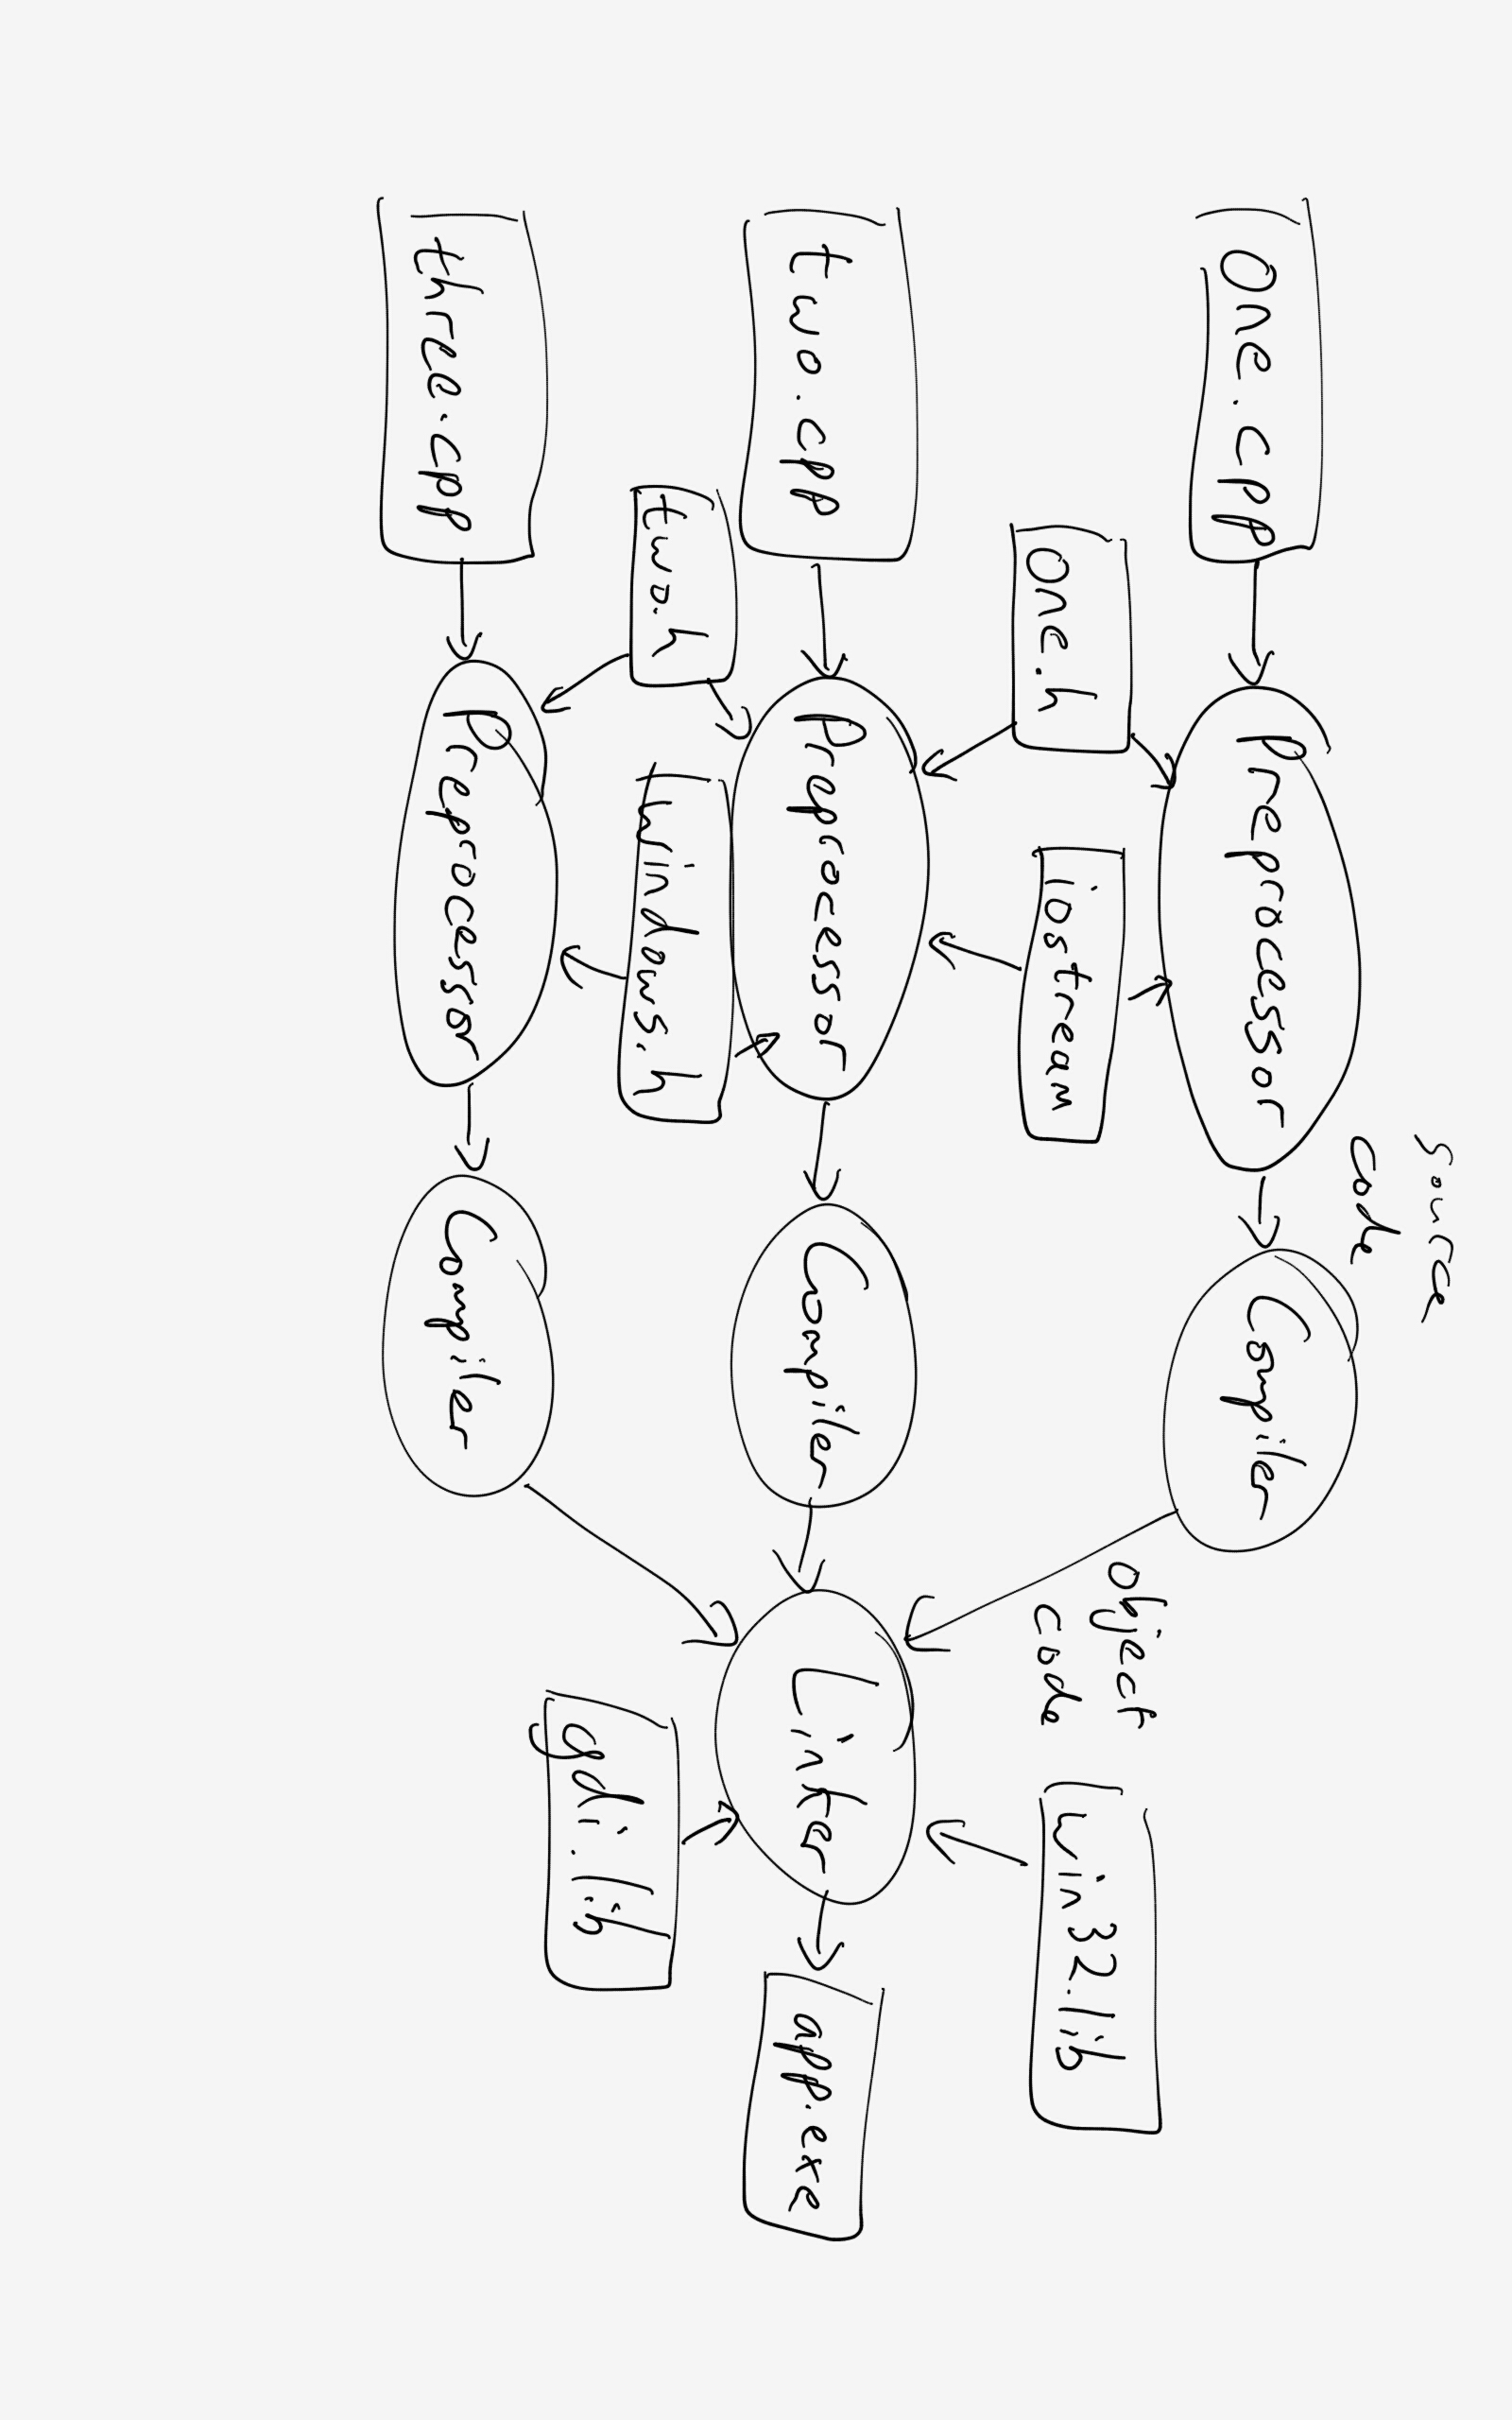
\includegraphics[height=\textwidth,angle=90]{compiler_sketch}
\end{frame}

\end{document}
